%! Author = chtompki
%! Date = 1/14/26
\documentclass[12pt]{amsart}
% Default margins are too wide all the way around. I reset them here
\setlength{\hoffset}{-.75in}
\setlength{\textwidth}{6.5in}
\setlength{\voffset}{-.5in}
\setlength{\textheight}{9.0in}
\usepackage{amsmath}
\usepackage{amssymb}
\usepackage{amsthm}
\usepackage{enumitem}
\usepackage{setspace}
\usepackage{graphicx}

\newenvironment{solution}
{\begin{proof}[Solution]}
{\end{proof}}

\title{Numerical Analysis\\Guided Lab 1}
\author{Rob Tompkins}
\date{\today}

\begin{document}
    \maketitle
    \date{\today}
    \begin{onehalfspace}
        % Problem 1
        \textbf{1.} Compute the absolute and relative error for
        \begin{displaymath}
            \sqrt{2} \approx 1 + \frac{24}{60} + \frac{51}{60^2} + \frac{10}{60^3}
        \end{displaymath}
        \begin{solution}
            Let's first compute the left and right hand side of the equation above using $x_{\text{approx}}$ to
            represent the approximate solution (RHS). Using matlab we see that
            \begin{eqnarray*}
                x & \approx & 1.41421356237, \text{ and} \\
                x_{\text{approx}} & = & 1.4142129630
            \end{eqnarray*}
            Let $\varepsilon_{\text{abs}}$ represent the absolute error, and $\varepsilon_{\text{rel}}$ represent the
            relative error. Then we have the following:
            \begin{eqnarray*}
                \varepsilon_{\text{abs}} & = & |\sqrt{2} - x_{\text{approx}} | \\
                & = & |1.41421356237 - 1.4142129630| = 5.99 \times 10^{-7}
            \end{eqnarray*}
            and we also see that:
            \begin{eqnarray*}
                \varepsilon_{\text{rel}} & = & \frac{\varepsilon_{abs}}{\sqrt{2}} \\
                & \approx & \frac{5.99\times 10^{-7}}{1.41421356237}\\
                & \approx & 4.24\times 10_{-7}
            \end{eqnarray*}
        \end{solution}

        % Problem 2
        \textbf{2.}
        The Newton-Raphason method for determining $\sqrt{a}$ follows from repeated
        iteration of
        \begin{displaymath}
            y_{n+1} = \frac{1}{2} \left(y_n + \frac{a}{y_n}\right)
        \end{displaymath}
        Show that $y = \sqrt{a}$ is the fixed point of this sequence.
        \begin{proof}
            To achieve $y = \sqrt{a}$ as a fixed point of our equation we will need to
            compare the error between the $n^{\text{th}}$ term and the $(n+1)^{\text{st}}$
            term.

            We begin by subtracting $\sqrt{a}$ from both sides of the equation and performing some
            algebraic manipulation. Consider
            \begin{eqnarray*}
                x_{n+1} - \sqrt{a} & = & \frac{1}{2} \left(x_n + \frac{a}{x_n}\right) - \sqrt{a} \\
                                   & = & \frac{x_n^2 - 2x_n\sqrt{a} + a}{2x_n} \\
                                   & = & \frac{(x_n - \sqrt{a})^2}{2x_n}
            \end{eqnarray*}
            Accordingly,
            \begin{eqnarray*}
                \lim_{n\rightarrow\infty} \frac{|x_{n+1} - \sqrt{a}|}{|x_n - \sqrt{a}} & = & \lim_{n\rightarrow\infty} \frac{1}{2x_n} \\
                 & = & \frac{1}{2\sqrt{a}}
            \end{eqnarray*}
            Hence the sequence generated by this scheme has order of convergence equal to 2 and asymptotic error constant
            $1/(2\sqrt{a})$.
        \end{proof}

        % Problem 3
        \textbf{3.} Create a script that implements Heron's algorithm (the formula in problem 1). It should take as the
        input: (1) the number $a$ to square root, (2) the initial guess $y_0$, and (3) the total number $N$ of iterations.
        In addition to outputting the approximate square root at each iteration. you may use a bulit-in functionas the
        ``exact'' answer for comparison. Plot bothe the relative error as a function of iteration for $N = 6$ on a
        log-log scale for $a = 2$. How sensitive is the result to y our initial guess of $y_0$?

        \begin{solution}
            Consider a function that we have in file ``problem3.m'' that we have below:
            \begin{verbatim}
                function [p,absError,relError] = fixpt(a,y,n)
                    % Input - a, the number to sqaure root
                    %       - y, the initial guess
                    %       - n, the number of iterations to run
                        p = y; % Initialize p with the initial guess
                        for k = 1:n
                            p_new = 0.5 * (p + a / p);
                            absError = abs(p_new - p);
                            relError = absError / abs(p_new);
                            if absError < 1e-10
                                break;
                            end
                            p = p_new;
                        end
                    end
            \end{verbatim}
            So we see our plot from the above results as:
            \begin{figure}[!ht]
                \centering
                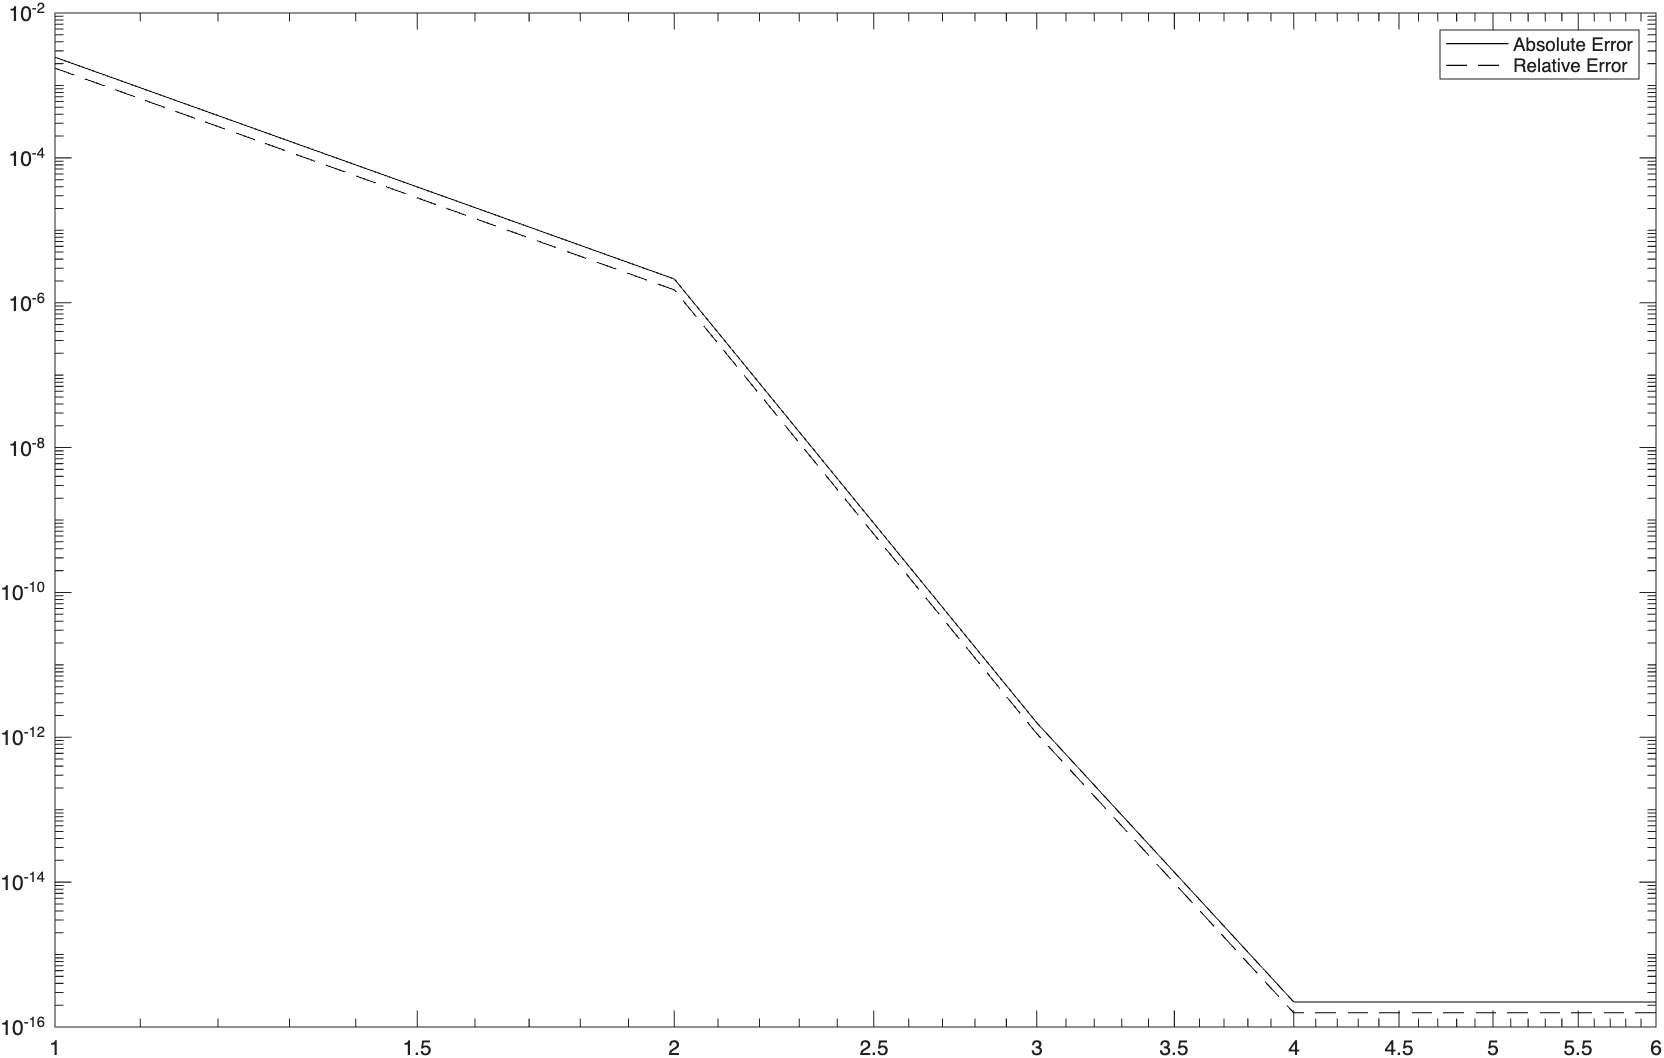
\includegraphics[scale=0.4]{Figure_1.png}
                \caption{Log-Log plot of the absolute and relative error for Newton Raphson for $N=6$, $y_0=1.5$}
            \end{figure}
            But, if we fiddle with the initial value for the answer we see different errors. Consider Figure 2 which shows
            the errors when we set $y_0 = 30$

            \begin{figure}[!ht]
                \centering
                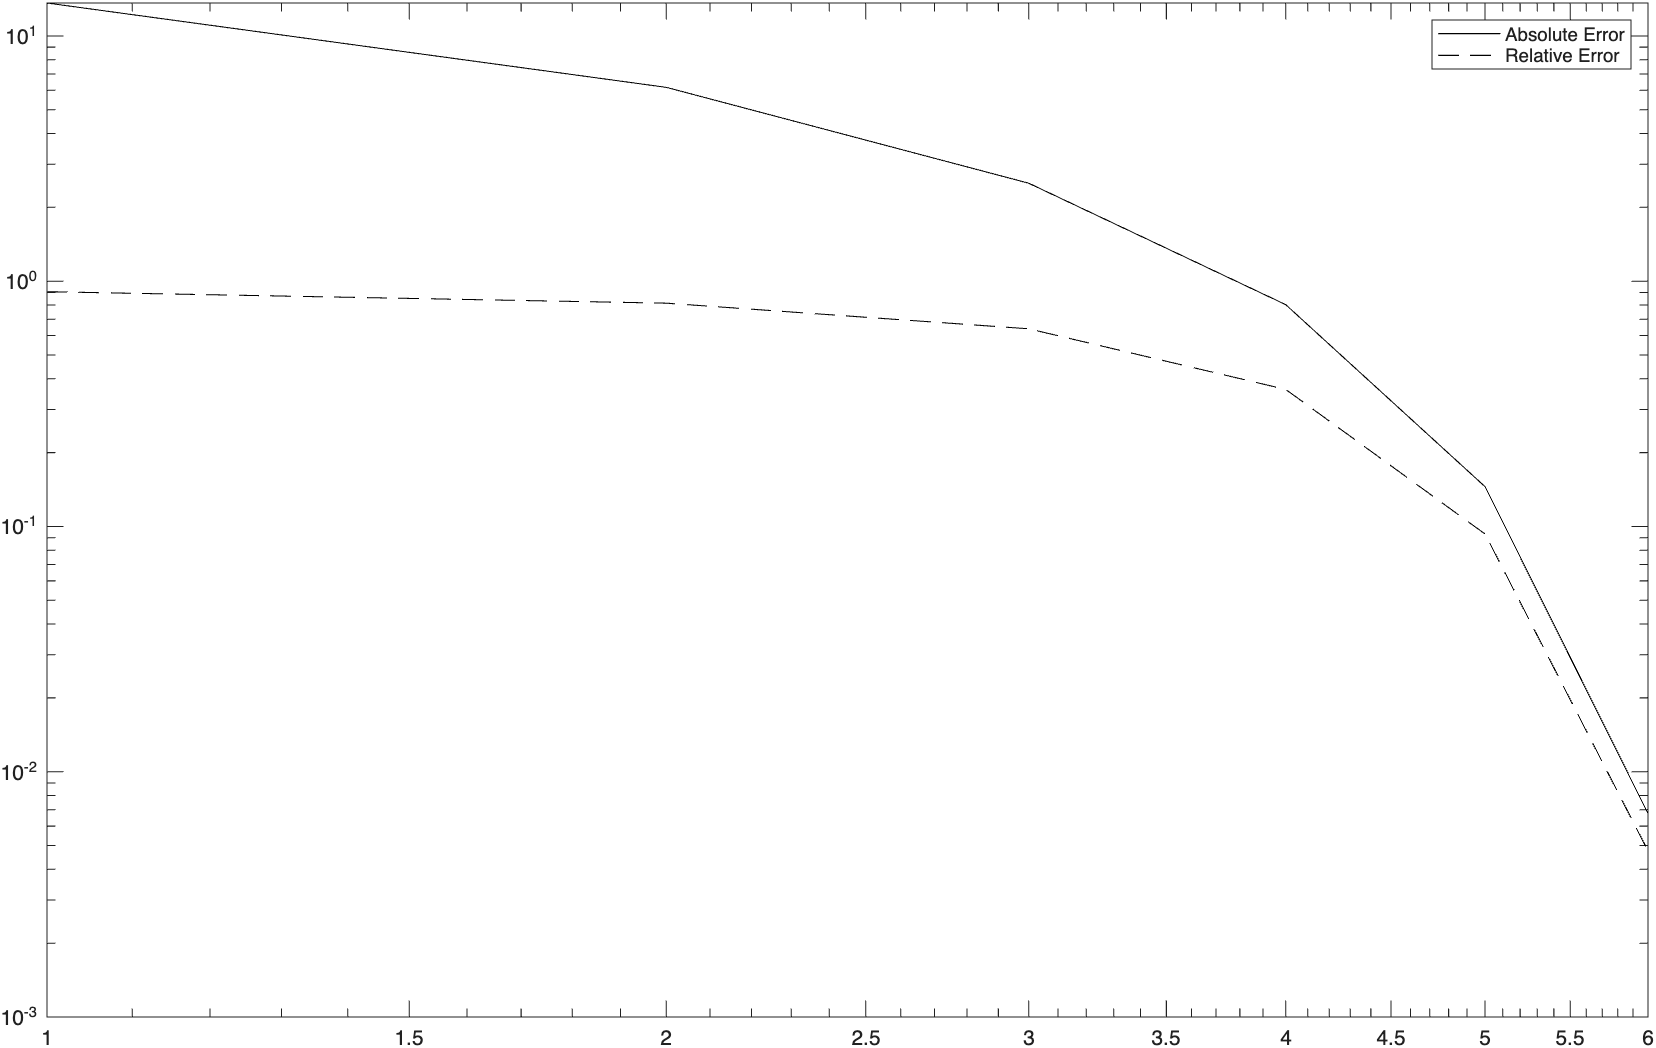
\includegraphics[scale=0.4]{Figure_2.png}
                \caption{Log-Log plot of the absolute and relative error for Newton Raphson for $N=6$, $y_0=30$}
            \end{figure}
            and we are done.
        \end{solution}

        % Problem 4
        \textbf{4.}
        \begin{solution}
            Problem 4
        \end{solution}

        % Problem 5
        \textbf{5.}
        \begin{solution}
            Problem 5
        \end{solution}

        % Problem 6
        \textbf{6.}
        \begin{solution}
            Problem 6
        \end{solution}

        % Problem 7
        \textbf{7.}
        \begin{solution}
            Problem 7
        \end{solution}

        % Problem 8
        \textbf{8.}
        \begin{solution}
            Problem 8
        \end{solution}

        % Problem 9
        \textbf{9.}
        \begin{solution}
            Problem 9
        \end{solution}

        % Problem 10
        \textbf{10.}
        \begin{solution}
            Problem 10
        \end{solution}



    \end{onehalfspace}
\end{document}
